\documentclass[aps,prl,reprint,superscriptaddress,amsmath,amssymb]{revtex4-2}
\usepackage{graphicx}
\usepackage[colorlinks=true,linkcolor=blue,citecolor=blue,urlcolor=blue]{hyperref}

\newcommand{\Tr}{\operatorname{Tr}}
\newcommand{\Reach}{\operatorname{Reach}}
\newcommand{\C}{\mathbb{C}}
\newcommand{\lean}[1]{\texttt{#1}}

\begin{document}

\title{Correlations Among Any Number of Identical Quantum Systems Can Always Be Created at Minimal Energy Cost}

\author{Ansh Mishra}
\email{ansh.mishra2025@gmail.com}
\affiliation{Independent researcher, Cumming, Georgia, USA}
\author{Aryan Senthilkumar}
\email{aryan.senthilk@gmail.com}
\affiliation{Independent researcher, Johns Creek, Georgia, USA}

\date{\today}

\begin{abstract}
Correlating identical quantum systems in thermal equilibrium costs energy, and thermodynamics bounds the correlations a
given energy can buy. The bound is attained if and only if a global unitary heats every system to one common thermal
state. For two systems such symmetrically thermalizing unitaries were conjectured in 2019 to exist in every dimension.
We prove this for every finite dimension, Hamiltonian, and temperature, and for any number of systems. The two-system
unitary is explicit, creates excitations in pairs, and is machine-checked in Lean.
\end{abstract}

\maketitle

Quantum thermodynamics asks which transformations of quantum systems are possible and at what
cost~\cite{HorodeckiOppenheim2013,Brandao2015,Goold2016,Vinjanampathy2016}. Its bounds acquire operational meaning
when they can be attained: Landauer's bound on the heat dissipated by erasure~\cite{Landauer1961,ReebWolf2014} and
bounds on the work extractable from nonequilibrium or correlated states~\cite{Allahverdyan2004,PerarnauLlobet2015} can
be approached by explicit protocols, and second laws that include correlations~\cite{Bera2017} refine what is
possible. Correlations are consumed by quantum technologies and reshape thermodynamic processes, even making heat flow
from a cold body to a hot one~\cite{Micadei2019}, but creating them from a thermal state costs
energy~\cite{Huber2015,Bruschi2015,Vitagliano2018}. Whether the minimal cost can be attained was known only in special
cases, which do not cover, for instance, two identical interacting many-body systems at arbitrary temperatures.

Consider two identical systems $A$ and $B$ with Hamiltonian $H$ in equilibrium with a bath at inverse temperature
$\beta$, so that their joint state is $\tau_\beta\otimes\tau_\beta$ with $\tau_\beta=e^{-\beta H}/\Tr e^{-\beta H}$.
An experimenter decouples them from the bath and applies a global unitary $U$. The state
$\tau_\beta\otimes\tau_\beta$ is completely passive~\cite{PuszWoronowicz1978,Lenard1978}, so every such operation
costs energy, and the question is how much correlation, measured by the mutual information $I(A{:}B)$, a given
amount of invested energy can buy~\cite{Huber2015,Bruschi2015}. Huber \textit{et al.}~\cite{Huber2015} showed that the
optimal trade-off is reached precisely when both final marginals equal one and the same hotter thermal state
$\tau_{\beta'}$, and they constructed such unitaries for equally spaced spectra (see also
Refs.~\cite{Jevtic2012,McKay2018}) and for sufficiently large temperature differences. Bakhshinezhad
\textit{et al.}~\cite{Bakhshinezhad2019} named them symmetrically thermalizing unitaries (STUs), proved their
existence for local dimension $d\le4$ and in the limit of infinitely many copies, and conjectured that they exist in
every dimension. Beyond $d=4$ only sufficient conditions were known, and the general case remained
open~\cite{Bakhshinezhad2019,Clivaz2020}.

Here we prove the conjecture. For every finite dimension, every Hamiltonian, and every pair of temperatures $T'\ge T$
there is a global unitary that heats both systems to exactly the same thermal state at temperature $T'$. We then
extend the result to any number of identical systems, so that the thermodynamic bound on the energy cost of
correlations is tight for every collection of identical finite-dimensional systems, including interacting many-body
systems. For two systems the proof is constructive and yields an explicit
optimal unitary with a transparent physical structure: it creates and destroys excitations only in pairs, as two-mode
squeezing does. We also observe that optimal correlation creation must generate entanglement once the target
temperature is high enough, and we show that a stronger, purely spectral version of the conjecture fails in every
dimension $d\ge4$. Because the argument combines combinatorial constructions with delicate analytic estimates, we have
formalized the complete existence proof for two systems in the Lean~4 proof assistant~\cite{Lean2021} with its
mathematical library Mathlib~\cite{Mathlib2020}.

\textit{Energy cost of correlations.}---Because the global entropy is invariant under unitaries, the correlations
created by $U$ are $\Delta I=\Delta S_A+\Delta S_B$, and the invested energy is $\Delta E=\Delta E_A+\Delta E_B$.
Define $\beta'$ by $\Delta E=2\Tr[H(\tau_{\beta'}-\tau_\beta)]$, and let $\rho'_A$ and $\rho'_B$ be the final
marginals. Then every global unitary obeys the identity
\begin{equation}\label{eq:identity}
2\bigl[S(\tau_{\beta'})-S(\tau_\beta)\bigr]-\Delta I=D(\rho'_A\Vert\tau_{\beta'})+D(\rho'_B\Vert\tau_{\beta'}),
\end{equation}
where $D$ is the quantum relative entropy~\cite{SM}. Since $D\ge0$, with equality only for equal arguments,
\begin{equation}\label{eq:bound}
\Delta I\le2\bigl[S(\tau_{\beta'})-S(\tau_\beta)\bigr],
\end{equation}
with equality if and only if both final marginals equal $\tau_{\beta'}$~\cite{Huber2015,Bakhshinezhad2019}. Creating a
given amount of mutual information thus costs at least the energy needed to heat both systems to the common
temperature at which their entropies have grown by the required amount [black curve in Fig.~\ref{fig:1}(b)]. The
bound is attained if and only if there is a unitary $U$ on $\C^d\otimes\C^d$ that is \emph{symmetrically
thermalizing} for $(H,\beta,\beta')$, that is,
\begin{equation}\label{eq:stu}
\Tr_B\bigl[U(\tau_\beta\otimes\tau_\beta)U^\dagger\bigr]=\Tr_A\bigl[U(\tau_\beta\otimes\tau_\beta)U^\dagger\bigr]
=\tau_{\beta'} .
\end{equation}
The symmetry of this requirement is what makes it hard. Each marginal separately can be heated to $\tau_{\beta'}$ in
many ways, but a single global unitary must do both at once while respecting the fixed spectrum of
$\tau_\beta\otimes\tau_\beta$. For two systems with different Hamiltonians the analogous statement
fails~\cite{Bakhshinezhad2019}. Which pairs of marginals are compatible with a given global spectrum is the quantum
marginal problem~\cite{Klyachko2004,Daftuar2005,Christandl2006}. Its answer is a convex polytope cut out by
complicated families of linear inequalities, and the symmetric thermal slice relevant here had not been characterized.

\begin{figure*}[t]
\centering
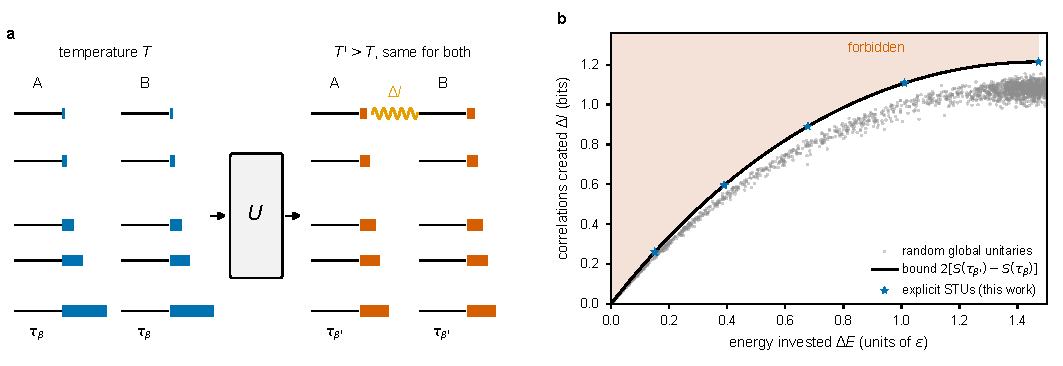
\includegraphics[width=\textwidth]{figures/fig1.pdf}
\caption{Creating correlations at the fundamental energy cost. (a)~Two identical systems start in the thermal state
$\tau_\beta$ at temperature $T$ (bars: level populations). A global unitary $U$ correlates them. It is optimal
exactly when both systems end up in the same thermal state $\tau_{\beta'}$ at a higher temperature $T'$; the
correlations are then $\Delta I=2[S(\tau_{\beta'})-S(\tau_\beta)]$. (b)~Mutual information $\Delta I$ created versus
energy $\Delta E$ invested, for a five-level system with energies $(0,0.62,1.05,1.83,2.41)\,\epsilon$ at
$\beta=1.3/\epsilon$. Black line: the bound~\eqref{eq:bound}; the shaded region above it is forbidden. Grey dots:
2500 random global unitaries $e^{-isK}$ with random Hermitian $K$ and random strength $s$; all lie below the bound.
Blue stars: the explicit STUs constructed in this work for $\beta'/\beta=0.85,0.65,0.45,0.25,0$; they lie on the
bound to machine precision (marginals exact to $2\times10^{-16}$).}
\label{fig:1}
\end{figure*}

\textit{Main result.}---Our main theorem settles the conjecture of Ref.~\cite{Bakhshinezhad2019}.

\textit{Theorem 1.} Let $d\ge1$, let $H$ be any Hermitian operator on $\C^d$, and let $\beta>0$ and
$0\le\beta'\le\beta$. Then there is a unitary $U$ on $\C^d\otimes\C^d$ that is symmetrically thermalizing for
$(H,\beta,\beta')$. If $|e_0\rangle,\dots,|e_{d-1}\rangle$ is an eigenbasis of $H$ with nondecreasing energies, $U$
can be chosen to be a real orthogonal matrix in the product basis $|e_i\rangle|e_j\rangle$ that commutes with
$N_A-N_B$, where $N=\sum_i i\,|e_i\rangle\langle e_i|$ counts the level index.

Degenerate spectra, the infinite-temperature target $\beta'=0$, and all intermediate temperatures are included.
Theorem~1 contains all previously known cases: equally spaced spectra, large temperature differences, and
$d\le4$~\cite{Huber2015,Bakhshinezhad2019}. Because $H$ is arbitrary, $A$ and $B$ may themselves be interacting
many-body systems. The physical consequence is that the curve in Fig.~\ref{fig:1}(b) is exactly the boundary of what
is achievable: for every pair of identical finite-dimensional systems, the minimal energy needed to create a given
amount of mutual information is the one dictated by Eq.~\eqref{eq:bound}, and it is achieved by a single global
unitary without ancillas, catalysts, or measurements. The unitary is explicit. The blue stars in Fig.~\ref{fig:1}(b)
were computed from it, and their marginals agree with $\tau_{\beta'}$ to within $2\times10^{-16}$.

\textit{Structure of the optimal protocol.}---Arrange the $d^2$ product levels $|e_i\rangle|e_j\rangle$ in a
$d\times d$ array (Fig.~\ref{fig:2}). The constructed $U$ acts separately on each of the $2d-1$ diagonals $j-i=t$ of
this array and therefore commutes with $N_A-N_B$: excitations are created and destroyed only in pairs, one in each
system. This is the symmetry of two-mode squeezing, the standard way of correlating two harmonic
modes~\cite{Weedbrook2012}, and of the thermofield double state $\sum_i q_i^{1/2}|e_i\rangle|e_i\rangle$, a pure
state with thermal marginals~\cite{TakahashiUmezawa1996}. Theorem~1 shows that this pair-creation structure suffices to
reach the optimum for arbitrary, non-equidistant spectra. Within each diagonal $U$ is a real rotation. It decomposes
into two-level rotations between product levels $|e_i\rangle|e_{i+t}\rangle$ and $|e_{i'}\rangle|e_{i'+t}\rangle$,
that is, into simultaneous (de-)excitations of both systems by the same number of levels. Two cells of one diagonal
never share a row or a column, so such rotations create no coherences that survive the partial trace. Both marginals
therefore remain diagonal in the energy eigenbasis, with populations given by the row and column sums of the final
population array [Fig.~\ref{fig:2}(c),(d)]. The diagonals refine the locally classical subspaces of
Ref.~\cite{Bakhshinezhad2019}: the subspace spanned by the levels $|e_j\rangle|e_{j+t \bmod d}\rangle$ is spanned by
the diagonals $t$ and $t-d$ (the latter is empty for $t=0$). Theorem~1 therefore shows that operating within these
subspaces suffices to reach every thermal target, which answers, for thermal targets, a question raised in
Ref.~\cite{Bakhshinezhad2019}.

\begin{figure*}[t]
\centering
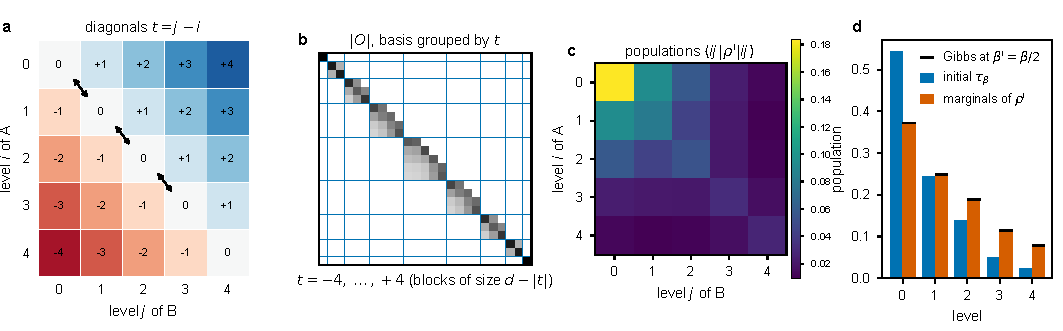
\includegraphics[width=\textwidth]{figures/fig2.pdf}
\caption{Structure of the optimal unitary, for the five-level system of Fig.~\ref{fig:1} and $\beta'=\beta/2$.
(a)~Product levels $|e_i\rangle|e_j\rangle$ arranged in a $5\times5$ array and labeled by the diagonal index $t=j-i$.
The constructed unitary acts within each diagonal and so conserves $N_A-N_B$. For $t=0$, for example, it rotates
$|00\rangle,|11\rangle,|22\rangle,\dots$ into each other (arrows), creating and destroying excitations in pairs.
(b)~Absolute values of the real orthogonal matrix $O$ in the product basis, grouped by $t$ (blocks of size $d-|t|$);
only 71 of its 625 entries are nonzero. (c)~Final populations $\langle ij|\rho'|ij\rangle$; the state is correlated,
but its row and column sums are thermal. (d)~Level populations of the initial marginals (blue), the final marginals
(orange; the two are identical), and the Gibbs distribution at $\beta'$ (black bars).}
\label{fig:2}
\end{figure*}

\textit{Proof strategy.}---Write $p_0\ge\dots\ge p_{d-1}>0$ for the thermal populations at $\beta$ and $q$ for those
at $\beta'$. By the Schur--Horn theorem~\cite{Schur1923,Horn1954}, a real rotation acting on one diagonal of the
array can produce exactly those populations on that diagonal that are majorized~\cite{MarshallOlkin2011} by the
initial products $p_ip_{i+t}$, and it can be built from Givens rotations~\cite{ChanLi1983}. An STU therefore exists
whenever there is a symmetric array $F$ whose diagonals are majorized by those of $p\otimes p$ and whose row sums are
$q$, and the set $\Reach(p)$ of row-sum vectors obtainable in this way is convex~\cite{SM}. As in the geometric
approach of Ref.~\cite{Bakhshinezhad2019}, it then suffices to reach $d$ explicit vectors whose convex hull contains
the thermal curve; Ref.~\cite{Bakhshinezhad2019} could reach its choice of vectors only for $d\le4$. We use instead
the \emph{clipped} states $w_k\propto\min(p,p_k)$: every vector $q\propto p^{\beta'/\beta}$, and more generally $g(p)$
for any concave nondecreasing $g$ with $g(0)\ge0$, is a convex combination of them~\cite{SM}. Reaching $w_k$ means
flattening the largest populations to a common value. We write $p\otimes p$ minus its clipped part as a nonnegative
combination of symmetric Young diagrams (squares and crosses) and replace every diagram by an \emph{interval
uniformization}: a symmetric matrix with entries between $0$ and $1$ that has the same diagonal sums as the diagram
but equal row sums. Because all pieces are nonincreasing along every diagonal, the majorization conditions
superpose, and an exact capacity identity of Hall type distributes the pieces over square subblocks of the array. The
core of the proof is an explicit construction of interval uniformizations for every block size and every interval of
Frobenius arm lengths, whose amplitudes are fixed by alternating harmonic sums~\cite{SM}. The entries of the
resulting unitary follow by Givens rotations from an explicit population array.

The vectors of the geometric approach of Ref.~\cite{Bakhshinezhad2019} are in fact reachable in every dimension, as
we also show. Combined with Kirwan's convexity theorem for moment maps~\cite{Kirwan1984}, which describes the full
quantum marginal polytope~\cite{Klyachko2004,Christandl2006}, this gives a second, nonconstructive proof~\cite{SM}.
Our main route avoids Kirwan's theorem and yields the explicit pair-creating unitary.

\textit{Any number of systems.}---For $N\ge2$ identical systems the relevant measure is the total correlation
$\sum_cS(\rho_c)-S(\rho)$. At energy cost $N\Tr[H(\tau_{\beta'}-\tau_\beta)]$ it is bounded by
$N[S(\tau_{\beta'})-S(\tau_\beta)]$, with equality if and only if every system ends in
$\tau_{\beta'}$~\cite{Huber2015}.

\textit{Theorem 2.} For all $N\ge2$, $d$, $H$, and $0\le\beta'\le\beta$ there is a unitary on $(\C^d)^{\otimes N}$
under which every one-body marginal of $\tau_\beta^{\otimes N}$ becomes $\tau_{\beta'}$.

For qubits such unitaries were known~\cite{PerarnauLlobet2015}. The circulant construction of Ref.~\cite{Huber2015}
extends to equally spaced spectra and large temperature differences, and for even $N$ Theorem~1 applied to disjoint
pairs suffices. For general $N$, we first construct, for each vector $v_k$ of the geometric approach, an explicit
unitary that brings all $N$ marginals to $v_k$ at once. Cells in which at least two systems occupy the $k+1$ most
populated levels are mixed by a common circulant, and the remaining cells are relabeled by cyclic shifts chosen by
bin packing. Kirwan's convexity theorem for $U(d)^N$~\cite{Kirwan1984,Christandl2014}, together with the fact that
every thermal target is a convex combination of the $v_k$~\cite{Bakhshinezhad2019}, then gives every target~\cite{SM}.
For $d\le3$ the construction is fully explicit and avoids Kirwan's theorem. The two-system unitary is followed by a
chain of two-body unitaries, each of which heats a fresh system to $\tau_{\beta'}$ while returning its partner's
marginal unchanged. This is a form of correlated catalysis~\cite{Boes2019,ShiraishiSagawa2021,Wilming2022} in which
the catalyst is a copy of the target state~\cite{SM}.

\textit{Entanglement and the role of thermal targets.}---Optimal correlation creation can require entanglement. The
final state has the global spectrum of $\tau_\beta\otimes\tau_\beta$, with largest eigenvalue $p_0^2$, while its
marginals have largest eigenvalue $q_0$. Separable states are more disordered globally than
locally~\cite{NielsenKempe2001}, so the optimal final state must be entangled whenever $p_0^2>q_0$: in
Fig.~\ref{fig:1} this holds for $T'>3.48\,T$, and for maximal correlations ($\beta'=0$) whenever $p_0>d^{-1/2}$. This
contrasts with work extraction, for which entanglement is not necessary~\cite{Hovhannisyan2013}.

One might expect a purely spectral statement: that every spectrum $q$ majorized by $p$, that is, every spectrum that a
unital channel on a single system can produce from $\tau_\beta$, is also reachable symmetrically from
$\tau_\beta\otimes\tau_\beta$. This stronger form holds for qutrits~\cite{Bakhshinezhad2019}, but it fails in every
dimension $d\ge4$~\cite{SM}. For $d=4$, for instance, $p=(0.94,0.05,0.005,0.005)$ and $q=(0.94,0.02,0.02,0.02)$ satisfy
$q\prec p$, but no unitary on $\C^4\otimes\C^4$ gives $\tau_\beta\otimes\tau_\beta$ two marginals with spectrum $q$. The
obstruction comes from the Ky Fan maximum principle~\cite{Bhatia1997}: the largest population of both marginals must
be kept, which forces the state into a block structure in which the remaining populations cannot be equalized.
Thermal targets escape this obstruction because they are mixtures of clipped states. Theorem~1 therefore rests on the
thermal (more generally, concave) form of the target, not on majorization alone.

\textit{Robustness and implementation.}---By Eq.~\eqref{eq:identity}, an imperfect implementation loses correlations
only through the relative entropies of its marginals to $\tau_{\beta'}$, which are quadratic in small deviations, so
the optimum is robust against small control errors. The two-level rotations of the protocol are two-body transitions
between $|e_ie_{i+t}\rangle$ and $|e_{i'}e_{i'+t}\rangle$ at frequencies $(E_{i'}+E_{i'+t}-E_i-E_{i+t})/\hbar$, which
are generically distinct for anharmonic spectra and could be driven by parametric two-body couplings of the kind used
for two-mode squeezing.

\textit{Machine-checked proof.}---To exclude errors in the combinatorial and analytic parts of the argument, we have
formalized the complete proof of the existence statement of Theorem~1 in Lean~4 with
Mathlib~\cite{Lean2021,Mathlib2020,repo}; the extension to $N$ systems relies on Kirwan's theorem, which is not
formalized. The
formal theorem \lean{STUProof.stu\_exists\_hermitian} states, for every $d$, every Hermitian matrix $H$, and every
$0\le\beta'\le\beta$ with $\beta>0$, that a unitary exists whose two marginals equal $\tau_{\beta'}$. The thermal state
is defined through Mathlib's matrix exponential, and the partial traces are defined explicitly. The files used by
this theorem contain about 7800 lines (the repository also holds superseded certificate-based proofs for $d\le40$),
and the whole development is checked in under an hour on a desktop computer. The final theorem depends only on Lean's
three standard axioms (propositional extensionality, choice, and quotient soundness); it contains no unproved
statements and does not trust compiled code. Formal verification has recently reached quantum information theory,
for example the generalized quantum Stein's lemma~\cite{Meiburg2025} and the rigidity of the CHSH
game~\cite{ZhaoYu2026}. Independent numerical and exact-arithmetic checks of the construction are reported in the
Supplemental Material~\cite{SM}.

\textit{Discussion.}---We have shown that the thermodynamic bound on the energy cost of correlations is attained for
any number of identical finite-dimensional quantum systems, by a global unitary that heats every system to one common
thermal state; for two systems the unitary is explicit. The minimal energy cost of correlations is thus known exactly,
for any spectrum, and for two systems it is achieved by a protocol with the pair-creation symmetry of two-mode
squeezing. Optimal protocols need not create
coherences between different values of $N_A-N_B$, can be built from real two-level rotations in the energy
eigenbasis, and must entangle the systems when the target temperature is high enough. Combined with the
counterexample to the spectral version of the problem, our results indicate that the thermal form of equilibrium
states imposes more structure on correlation creation than majorization alone.

Several questions remain open. For an odd number of systems with $d\ge4$ levels, an explicit construction that avoids
Kirwan's theorem is not known, and infinite-dimensional systems with arbitrary spectra are not covered. For systems with different Hamiltonians the symmetric formulation fails~\cite{Bakhshinezhad2019},
and the optimal trade-off is not known in general. Further directions include the fluctuations of the work cost of
optimal correlation creation~\cite{McKay2018}, the extremal correlations attainable in closed
evolutions~\cite{Jevtic2012}, and the minimal entanglement that optimal protocols require. More broadly, this work
shows that interactive theorem provers can certify results in quantum thermodynamics down to the last analytic
estimate.

\textit{Data availability.}---The Lean~4 formalization, the independent exact checkers, the verification logs, and
the script that computes the explicit unitaries and produces the figures are openly available~\cite{repo}.

\begin{acknowledgments}
We thank the developers of Lean and the Mathlib community for the software on which the formal verification is
built.

\textit{Use of AI tools.}---The large language model Claude (Anthropic; Opus models, accessed through Claude Code)
was used extensively, at the authors' direction, to develop and check the mathematical arguments, write the Lean
formalization and the verification code, produce the figures, and draft and edit the text. Its output was checked
by the authors; in addition, the existence proof is verified by the Lean kernel and the construction by independent
exact-arithmetic computations. The authors take full responsibility for the content of this Letter.
\end{acknowledgments}

\begin{thebibliography}{42}
\bibitem{HorodeckiOppenheim2013} M.~Horodecki and J.~Oppenheim, Fundamental limitations for quantum and nanoscale thermodynamics, Nat. Commun. \textbf{4}, 2059 (2013).
\bibitem{Brandao2015} F.~Brand\~{a}o, M.~Horodecki, N.~Ng, J.~Oppenheim, and S.~Wehner, The second laws of quantum thermodynamics, Proc. Natl. Acad. Sci. U.S.A. \textbf{112}, 3275 (2015).
\bibitem{Goold2016} J.~Goold, M.~Huber, A.~Riera, L.~del Rio, and P.~Skrzypczyk, The role of quantum information in thermodynamics---a topical review, J. Phys. A \textbf{49}, 143001 (2016).
\bibitem{Vinjanampathy2016} S.~Vinjanampathy and J.~Anders, Quantum thermodynamics, Contemp. Phys. \textbf{57}, 545 (2016).
\bibitem{Landauer1961} R.~Landauer, Irreversibility and heat generation in the computing process, IBM J. Res. Dev. \textbf{5}, 183 (1961).
\bibitem{ReebWolf2014} D.~Reeb and M.~M. Wolf, An improved Landauer principle with finite-size corrections, New J. Phys. \textbf{16}, 103011 (2014).
\bibitem{Allahverdyan2004} A.~E. Allahverdyan, R.~Balian, and T.~M. Nieuwenhuizen, Maximal work extraction from finite quantum systems, Europhys. Lett. \textbf{67}, 565 (2004).
\bibitem{PerarnauLlobet2015} M.~Perarnau-Llobet \textit{et al.}, Extractable work from correlations, Phys. Rev. X \textbf{5}, 041011 (2015).
\bibitem{Bera2017} M.~N. Bera, A.~Riera, M.~Lewenstein, and A.~Winter, Generalized laws of thermodynamics in the presence of correlations, Nat. Commun. \textbf{8}, 2180 (2017).
\bibitem{Micadei2019} K.~Micadei \textit{et al.}, Reversing the direction of heat flow using quantum correlations, Nat. Commun. \textbf{10}, 2456 (2019).
\bibitem{Huber2015} M.~Huber \textit{et al.}, Thermodynamic cost of creating correlations, New J. Phys. \textbf{17}, 065008 (2015).
\bibitem{Bruschi2015} D.~E. Bruschi, M.~Perarnau-Llobet, N.~Friis, K.~V. Hovhannisyan, and M.~Huber, Thermodynamics of creating correlations: Limitations and optimal protocols, Phys. Rev. E \textbf{91}, 032118 (2015).
\bibitem{Vitagliano2018} G.~Vitagliano, C.~Kl\"{o}ckl, M.~Huber, and N.~Friis, Trade-off between work and correlations in quantum thermodynamics, in \textit{Thermodynamics in the Quantum Regime}, edited by F.~Binder, L.~A. Correa, C.~Gogolin, J.~Anders, and G.~Adesso (Springer, Cham, 2018), pp.~731--750.
\bibitem{PuszWoronowicz1978} W.~Pusz and S.~L. Woronowicz, Passive states and KMS states for general quantum systems, Commun. Math. Phys. \textbf{58}, 273 (1978).
\bibitem{Lenard1978} A.~Lenard, Thermodynamical proof of the Gibbs formula for elementary quantum systems, J. Stat. Phys. \textbf{19}, 575 (1978).
\bibitem{Jevtic2012} S.~Jevtic, D.~Jennings, and T.~Rudolph, Maximally and minimally correlated states attainable within a closed evolving system, Phys. Rev. Lett. \textbf{108}, 110403 (2012).
\bibitem{McKay2018} E.~McKay, N.~A. Rodr\'{\i}guez-Briones, and E.~Mart\'{\i}n-Mart\'{\i}nez, Fluctuations of work cost in optimal generation of correlations, Phys. Rev. E \textbf{98}, 032132 (2018).
\bibitem{Bakhshinezhad2019} F.~Bakhshinezhad \textit{et al.}, Thermodynamically optimal creation of correlations, J. Phys. A \textbf{52}, 465303 (2019).
\bibitem{Clivaz2020} F.~Clivaz, Optimal manipulation of correlations and temperature in quantum thermodynamics, Ph.D. thesis, University of Geneva, 2020, \href{https://arxiv.org/abs/2012.04321}{arXiv:2012.04321}.
\bibitem{Lean2021} L.~de Moura and S.~Ullrich, The Lean 4 theorem prover and programming language, in \textit{Automated Deduction -- CADE 28}, edited by A.~Platzer and G.~Sutcliffe (Springer, Cham, 2021), pp.~625--635.
\bibitem{Mathlib2020} The mathlib Community, The Lean mathematical library, in \textit{Proceedings of the 9th ACM SIGPLAN International Conference on Certified Programs and Proofs} (ACM, New York, 2020), pp.~367--381.
\bibitem{SM} See Supplemental Material at [URL will be inserted by publisher] for the derivation of Eq.~(1), the complete proof of Theorem~1 with all lemmas and an overview figure of its architecture, the reachability of the vectors of the geometric approach and the resulting second proof via Kirwan's theorem, the counterexample to the spectral form, the correspondence between the proof and the Lean formalization, the proof of Theorem~2 for any number of systems and its formalization, and the independent computer checks.
\bibitem{Klyachko2004} A.~A. Klyachko, Quantum marginal problem and representations of the symmetric group, \href{https://arxiv.org/abs/quant-ph/0409113}{arXiv:quant-ph/0409113}.
\bibitem{Daftuar2005} S.~Daftuar and P.~Hayden, Quantum state transformations and the Schubert calculus, Ann. Phys. (N.Y.) \textbf{315}, 80 (2005).
\bibitem{Christandl2006} M.~Christandl and G.~Mitchison, The spectra of quantum states and the Kronecker coefficients of the symmetric group, Commun. Math. Phys. \textbf{261}, 789 (2006).
\bibitem{Weedbrook2012} C.~Weedbrook \textit{et al.}, Gaussian quantum information, Rev. Mod. Phys. \textbf{84}, 621 (2012).
\bibitem{TakahashiUmezawa1996} Y.~Takahashi and H.~Umezawa, Thermo field dynamics, Int. J. Mod. Phys. B \textbf{10}, 1755 (1996).
\bibitem{Schur1923} I.~Schur, \"{U}ber eine Klasse von Mittelbildungen mit Anwendungen auf die Determinantentheorie, Sitzungsber. Berl. Math. Ges. \textbf{22}, 9 (1923).
\bibitem{Horn1954} A.~Horn, Doubly stochastic matrices and the diagonal of a rotation matrix, Am. J. Math. \textbf{76}, 620 (1954).
\bibitem{MarshallOlkin2011} A.~W. Marshall, I.~Olkin, and B.~C. Arnold, \textit{Inequalities: Theory of Majorization and Its Applications}, 2nd ed. (Springer, New York, 2011).
\bibitem{ChanLi1983} N.~N. Chan and K.-H. Li, Diagonal elements and eigenvalues of a real symmetric matrix, J. Math. Anal. Appl. \textbf{91}, 562 (1983).
\bibitem{Kirwan1984} F.~Kirwan, Convexity properties of the moment mapping, III, Invent. Math. \textbf{77}, 547 (1984).
\bibitem{Christandl2014} M.~Christandl, B.~Doran, S.~Kousidis, and M.~Walter, Eigenvalue distributions of reduced density matrices, Commun. Math. Phys. \textbf{332}, 1 (2014).
\bibitem{Boes2019} P.~Boes, J.~Eisert, R.~Gallego, M.~P. M\"uller, and H.~Wilming, Von Neumann entropy from unitarity, Phys. Rev. Lett. \textbf{122}, 210402 (2019).
\bibitem{ShiraishiSagawa2021} N.~Shiraishi and T.~Sagawa, Quantum thermodynamics of correlated-catalytic state conversion at small scale, Phys. Rev. Lett. \textbf{126}, 150502 (2021).
\bibitem{Wilming2022} H.~Wilming, Correlations in typicality and an affirmative solution to the exact catalytic entropy conjecture, Quantum \textbf{6}, 858 (2022).
\bibitem{NielsenKempe2001} M.~A. Nielsen and J.~Kempe, Separable states are more disordered globally than locally, Phys. Rev. Lett. \textbf{86}, 5184 (2001).
\bibitem{Hovhannisyan2013} K.~V. Hovhannisyan, M.~Perarnau-Llobet, M.~Huber, and A.~Ac\'{\i}n, Entanglement generation is not necessary for optimal work extraction, Phys. Rev. Lett. \textbf{111}, 240401 (2013).
\bibitem{Bhatia1997} R.~Bhatia, \textit{Matrix Analysis} (Springer, New York, 1997).
\bibitem{repo} A.~Mishra and A.~Senthilkumar, Symmetrically thermalizing unitaries: Lean~4 formalization, certificates and verification logs, \url{https://github.com/anshM123/symmetrically-thermalizing-unitaries} (2026).
\bibitem{Meiburg2025} A.~Meiburg, L.~A. Lessa, and R.~R. Soldati, A formalization of the generalized quantum Stein's lemma in Lean, \href{https://arxiv.org/abs/2510.08672}{arXiv:2510.08672}.
\bibitem{ZhaoYu2026} T.~Zhao and N.~Yu, Formalizing CHSH rigidity in Lean 4, \href{https://arxiv.org/abs/2604.03884}{arXiv:2604.03884}.
\end{thebibliography}


\end{document}
